% GENERATED FILE -- DO NOT EDIT. Edit report.md and run `make report` from the
% repository root (writeups/midway_report/build_report.py), which regenerates
% this file, the figures, and report.pdf. Template: iclr_pandoc.latex.
\documentclass{article}
\PassOptionsToPackage{hyphens}{url}
\usepackage{iclr2025_conference,times}
\usepackage{hyperref}
\usepackage{xurl}

\hypersetup{hidelinks,
  pdftitle={Is the Gap an Interface Gap? An Agent Tool Interfaces for Data Catalogs},
  pdfauthor={Alex Feng}}

% Additions pandoc output needs (tables, figures, tight lists).
\usepackage{longtable,booktabs,array,calc}
\usepackage{etoolbox}
\makeatletter
\patchcmd\longtable{\par}{\if@noskipsec\mbox{}\fi\par}{}{}
\makeatother
\usepackage{graphicx}
\makeatletter
\newsavebox\pandoc@box
\newcommand*\pandocbounded[1]{%
  \sbox\pandoc@box{#1}%
  \Gscale@div\@tempa{\textheight}{\dimexpr\ht\pandoc@box+\dp\pandoc@box\relax}%
  \Gscale@div\@tempb{\linewidth}{\wd\pandoc@box}%
  \ifdim\@tempb\p@<\@tempa\p@\let\@tempa\@tempb\fi
  \ifdim\@tempa\p@<\p@\scalebox{\@tempa}{\usebox\pandoc@box}%
  \else\usebox{\pandoc@box}%
  \fi%
}
\def\fps@figure{htbp}
\makeatother
\providecommand{\tightlist}{%
  \setlength{\itemsep}{0pt}\setlength{\parskip}{0pt}}
\newcounter{none}
\setlength{\LTcapwidth}{\textwidth}

% CS329Z midway report, generated from report.md.

\title{[Midway Report] Is the Gap an Interface Gap?\\ An Agent Tool Interfaces for Data Catalogs}
\author{Alex Feng}
\iclrfinalcopy

\begin{document}
\maketitle
\vspace{-0.3in}
\lhead{CS329Z: Engineering AI Agents -- Midway Report}

\section{Problem Statement (Problem Specification)}\label{sec:problem}

Maintainers of a dbt-backed lakehouse need catalog metadata (ownership, grain, filters, lifecycle state) that stays trustworthy as models evolve, but it drifts from the code---annotations ``can become outdated or incorrect'' as data models evolve \citep{lakafosis2025meta}---and the evidence for a correction is scattered across catalog metadata, SQL, lineage, tests, and the data. We are building a \emph{catalog steward} for them with two triggers over one workflow: \emph{remediation} of existing hygiene debt and \emph{change review} of a proposed contribution. Our question: \textbf{does a specialized evidence-gathering, risk-aware action, and verification workflow produce more complete, grounded, and safe maintenance outcomes than static checks or a generic coding agent with the same raw repository and warehouse access?}

\section{Methodology}\label{sec:method}

\subsection{Environment \& Data}\label{sec:env}

\textbf{Environment.} The environment is a repository-local dbt Core project \citep{dbtcore} backed by DuckDB \citep{raasveldt2019duckdb} through the dbt-duckdb adapter. Three small synthetic seed tables (5 customers, 8 orders, 10 order items) feed a staging model and two aggregates (\texttt{customer\_orders}, \texttt{daily\_revenue}), with schema documentation, dbt tests, and a JSON catalog snapshot; a compact \texttt{catalog/overrides.json} sidecar injects controlled metadata changes. It is a reproducible test bed, not evidence about production warehouses. Each episode copies the clean base, applies a debt or change overlay, generates the diff, and builds the project, so every condition starts from the same state.

\textbf{Hygiene contract.} A versioned contract (\texttt{design/hygiene\_contract.yaml}, v0.1.0, validated by a JSON Schema) bounds the task to five issue types: missing required metadata, SQL/metadata drift, grain or join drift, unsupported reliability claims, and lifecycle drift. Each type names its required evidence, allowed and forbidden action classes, and verification. Limits: 20 assets, two lineage hops, five findings, and 10,000 probed rows; deleting assets, changing access policies, mutating a live catalog, inventing business semantics, and unbounded queries are forbidden.

\textbf{Evaluation data and ground truth.} The pilot suite has ten hand-constructed, versioned episodes (\texttt{data/episodes/manifest.yaml}): four \emph{remediation} cases (a stale revenue-filter description, wrong customer-order grain, a missing owner, and a legacy copy still marked active and canonical), four \emph{flawed change} cases (a changed revenue filter, a changed grain without updated grain metadata or tests, a new undocumented model, and a rename without a lifecycle transition), and two \emph{clean controls} (a documented new model and a documented revenue metric). For each episode the manifest records the expected \texttt{(issue\_type,\ asset)} findings, required evidence, \emph{sets} of acceptable and unsafe actions, postconditions, and intended checks. Action sets let an escalation count as correct where business meaning is uncertain (e.g.~in the filter-drift case, proposing a description fix is acceptable but editing the SQL to match stale prose is unsafe); clean controls make spurious findings measurable.

\textbf{Success criteria and metrics.} The scorer (\texttt{midpoint-score-v1}) matches findings to the manifest exactly at the \texttt{(issue\_type,\ asset)} level. An episode \emph{succeeds} only with no missed and no extra finding, no action outside the issue type's allowed classes, no recorded verification failure, and a complete run. It also records precision, recall, action and evidence validity, patches, escalations, cost, and turns. Known limits: evidence validity checks that cited IDs resolve, not that the evidence supports the claim; the action score checks permitted classes, not the episode-specific acceptable and unsafe actions; and postconditions are not checked. We therefore audit every trace by hand before reading score gaps as quality or safety gaps.

\subsection{Methods}\label{sec:methods}

\textbf{Shared workflow and evidence tools.} Both triggers run the same inspect--plan--act--verify state machine; change review additionally collects the diff. For the scoped assets, the steward builds an evidence bundle from catalog metadata, the dbt schema and manifest, model SQL with facts parsed by SQLGlot \citep{mao_sqlglot} (sources, filters, joins, aggregates, grouping, grain candidates), one-hop lineage, and bounded profiles. Following the view that purpose-built agent--computer interfaces matter \citep{yang2024sweagent}, every evidence item carries a stable content-hashed ID and provenance pointer, and absent metadata is explicit \texttt{present:\ false} evidence. During planning the model may call nine schema-checked, read-only tools (e.g.~two-hop lineage, bounded profiles, confined file reads). It returns at most five prioritized findings, each with claim, confidence, impact, evidence, and action.

\textbf{Risk-aware action policy.} Before anything executes, a validator checks the plan schema, in-scope assets, supported issue types, each issue type's required evidence families, action permissions, and that every cited evidence ID resolves. Actions fall into three classes: a \emph{patch} for evidence-backed, reversible technical metadata; a \emph{proposal} that leaves semantic or organizational decisions to a reviewer; and a \emph{report} when no action is justified. Patches touch only five catalog fields in the episode-local override file, never a live catalog.

\textbf{Verification and ledger.} For a patch the steward emits a unified diff, applies it inside the episode, checks that the catalog field now equals the value the model declared and that \texttt{dbt\ parse} succeeds, and otherwise restores the file and records a verification failure. This is weak: \texttt{dbt\ parse} does not read \texttt{catalog/}, and the contract's per-issue checks (e.g.~comparing metadata to parsed SQL, rerunning a uniqueness probe) do not run yet. Proposals and reports get permission and evidence checks only; an append-only ledger records findings, evidence, actions, and checks.

\textbf{Conditions.} The frozen configuration (\texttt{experiments/configs/midpoint\_v1.yaml}, v1.2.0) defines three conditions. (1) \emph{Static checks}: required catalog/schema fields plus actual dbt test results, with no SQL parsing or semantic inference. (2) \emph{Generic agent}: the same model, repository, built warehouse, budgets, and output schema, but only four raw operations (list files, read a file, read the diff, bounded read-only SQL) and the issue labels, without the evidence bundle, per-issue rules, or verification. (3) \emph{Steward}: the full workflow above. Both model conditions use \texttt{openai/gpt-6-luna} with reasoning effort low, temperature 0, a 4,096-token limit, at most 12 turns, one reply protocol, and one identical repair turn for a final answer that fails validation (prompts \texttt{generic-hygiene-v3}, \texttt{specialized-steward-v3}). Each episode is one sample (temperature is likely ignored by this reasoning model). Generic-agent patches are plan text only, never applied, while a failed steward verification loses the episode. The comparison tests workflow, evidence, and tools together.

\subsection{What Did Not Work, and Pivots}\label{sec:pivots}

\textbf{From catalog QA to a hygiene steward.} The proposal planned a 180-question catalog QA benchmark on a Docker Unity Catalog/Iceberg stack, swept across five harnesses and many models. After feedback that the motivation was narrow and the sweep too ambitious, we pivoted to the maintenance problem underneath, with two headline outcomes (a verified repair and a prevented regression), on a local fixture.

\textbf{Evaluator defects and a label leak, fixed before any paid run.} An audit of the first static run fixed two scorer defects (stale \texttt{dbt\ test} results reused; duplicate findings inflating action rates). A scripted-model preflight of the paid pipeline fixed lost transcripts and costs on failed runs and found an \emph{episode-label leak} through three channels: the steward prompt contained the episode ID (e.g.~\texttt{rem\_daily\_revenue\_filter\_drift}, which names the expected finding), workspace paths that dbt copies into readable artifacts embedded it too, and DuckDB file readers in the generic agent's SQL tool could have read the label manifest itself. Opaque workspace tokens, path rewriting, and disabled DuckDB external access fixed it, and a test asserts that no label reaches either condition's model input.

\textbf{Protocol repair, and a failure left unfixed.} In a paid two-episode smoke run the model copied the wrapper object from the reply-format example, the main source of rejected replies; because the generic agent makes more calls, this penalized it more. We fixed the shared example and error messages and added the identical repair turn (config 1.2.0); a smoke rerun passed a pre-set gate, and the pilot then ran once. The pilot exposed a new failure---the generic agent batching several tool calls, once with invented results, into one reply---which we left unfixed under a pre-committed no-iteration rule, to avoid tuning prompts on the evaluation set.

\section{Results (Summary of Progress)}\label{sec:results}

\textbf{Completed work and setup.} Everything in Section~\ref{sec:method} is implemented and covered by 93 deterministic tests that make no model calls. The pilot ran each condition once on the ten episodes from fresh fixtures under config 1.2.0: 30 runs, 0 errors, about 8.5 minutes, \$0.0172 of model spend (\$0.0244 for the whole project). Four of the 20 model records (the two demo episodes in both model conditions) are exact cache replays of the 1.2.0 smoke rerun, not new samples. We audited every trace by hand (\texttt{analysis.md}).

\begin{longtable}[]{@{}lrrrrrrrr@{}}
\caption{Episode successes by condition and category (remediation, flawed change, clean control), finding counts, and micro precision/recall; an errored run counts its expected findings as missed. Source: \protect\texttt{experiments/results/midpoint\_v1\_2\_pilot/summary.json}.}\label{tbl:results}\tabularnewline
\toprule\noalign{}
Condition & Remed. & Flawed & Clean & All & TP/FP/FN & Micro P/R & Errors & Cost (\$) \\
\midrule\noalign{}
\endfirsthead
\toprule\noalign{}
Condition & Remed. & Flawed & Clean & All & TP/FP/FN & Micro P/R & Errors & Cost (\$) \\
\midrule\noalign{}
\endhead
\bottomrule\noalign{}
\endlastfoot
Static checks & 1/4 & 1/4 & 2/2 & 4/10 & 4/0/6 & 1.00/0.40 & 0 & 0.00 \\
Generic agent & 2/4 & 1/4 & 2/2 & 5/10 & 5/4/5 & 0.56/0.50 & 0 & 0.01 \\
Steward & 2/4 & 3/4 & 0/2 & 5/10 & 9/6/1 & 0.60/0.90 & 0 & 0.01 \\
\end{longtable}

\begin{figure}
\centering
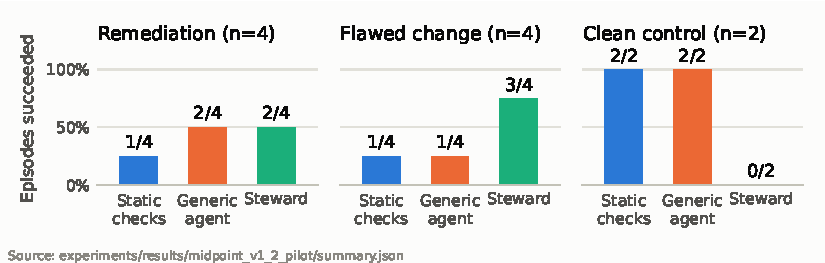
\includegraphics[width=1\linewidth,height=\textheight,keepaspectratio,alt={Episode success by condition and category, one run per episode. The steward leads on flawed changes and fails both clean controls, which static checks and the generic agent pass.}]{figures/success_by_category.pdf}
\caption{Episode success by condition and category, one run per episode. The steward leads on flawed changes and fails both clean controls, which static checks and the generic agent pass.}\label{fig:success}
\end{figure}

\begin{figure}
\centering
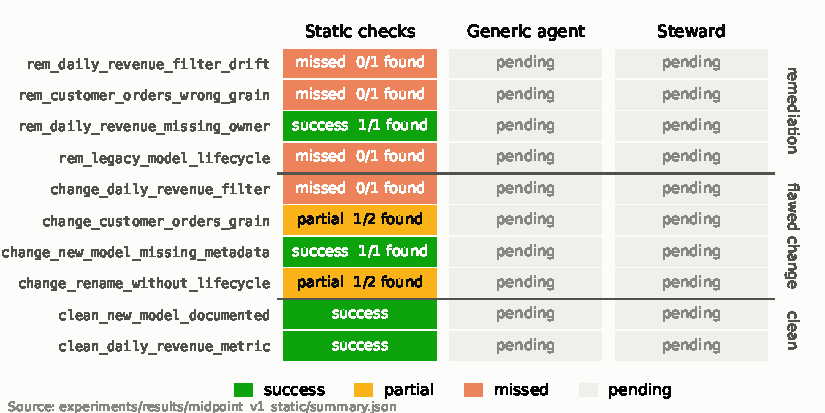
\includegraphics[width=0.88\linewidth,height=\textheight,keepaspectratio,alt={Per-episode outcome. Partial: at least one expected finding matched but the episode failed (a miss, an extra finding, or a disallowed action). Missed: no expected finding matched. False alarm: any finding on a clean control, true or not (both steward flags are real, unlabelled fixture gaps).}]{figures/outcome_grid.pdf}
\caption{Per-episode outcome. \emph{Partial}: at least one expected finding matched but the episode failed (a miss, an extra finding, or a disallowed action). \emph{Missed}: no expected finding matched. \emph{False alarm}: any finding on a clean control, true or not (both steward flags are real, unlabelled fixture gaps).}\label{fig:grid}
\end{figure}

\textbf{Interpretation.} On ten author-built fixtures with one run each, the steward matched 9 of 10 expected issues, against 5 for the generic agent and 4 for static checks (Table~\ref{tbl:results}), and every steward claim cited real evidence. It still only tied the generic agent on episode success (5/10 each; static 4/10) because it over-reported: six extra findings, three of them real but unlabelled fixture gaps, including both clean-control flags (an undocumented seed, and a model description that omits a newly documented metric). The generic agent's score is fragile the other way: one success is a pass in which it read no files; one failure rested on tool output it invented, which still passed the ID-based evidence check; and one run approved the refund regression without reading anything, an unsafe action the scorer cannot see. Under alternative label decisions the audit's sensitivity range is steward 7/10, generic 4/10, and static 3/10; this shows how much the headline rests on labels and is not a rescoring.

\textbf{What the comparison does not isolate.} The conditions differ by more than prompting: only the steward gets a pre-collected evidence bundle, the per-issue action contract, and a validator that enforces it, so its 14 model calls against the generic agent's 65, and its unsafe-action rate, are not like-for-like. On the wrong-grain episode both agents made the same grain patch; the steward avoided the penalty only because it labelled the problem SQL/metadata drift, where patches are allowed. Its three applied patches were correct on manual inspection, but its verification checks only the written value and \texttt{dbt\ parse}, not the manifest's semantic checks. Protocol scaffolding also weighs more on the generic agent: 7 of its 10 runs had a rejected reply, against 2 of 10 for the steward. We make no general or statistical claim.

\section{Assets}\label{sec:assets}

\textbf{Repository:} \mbox{\url{https://github.com/alfenn/agentic-catalog-interface}} \citep{feng2026repo}: \texttt{README.md} (setup, reproduction), \texttt{src/catalog\_steward/}, \texttt{data/} (fixture, episodes), and \texttt{experiments/results/midpoint\_v1\_2\_pilot/} (pilot results, audit \texttt{analysis.md}). Midpoint demo video: \textbf{{[}VIDEO URL TO BE ADDED{]}}.

\section{Timeline (Summary of Progress: Next Steps and Risks)}\label{sec:timeline}

\textbf{Milestones.} Course deadlines are Demo Day on December 9 and the final 8-page report on December 11; intermediate dates are our targets.

\begin{itemize}
\tightlist
\item
  \emph{By November 13:} a new frozen episode version: documented seeds, truly clean controls, an issue-type precedence rule checked independently of the model's label, and human review of the AI-built labels.
\item
  \emph{By November 20:} postcondition-based success and episode-level unsafe-action checks; real per-issue patch verification; a batching-robust protocol.
\item
  \emph{By December 4:} a checklist baseline, tool-versus-workflow ablations, and growth toward 30--50 audited episodes.
\item
  \emph{December 9 and 11:} live demo of both modes; final report.
\end{itemize}

\textbf{Obstacles and concerns.} No credential or pipeline blocker remains. The main concern is validity: label choices and protocol behaviour move results as much as the workflow, so fixes go into a new frozen version, not a rescoring.

\textbf{Risks and mitigations.} \emph{Scope growth:} a frozen five-type contract with hard limits. \emph{Ambiguous ground truth} (seen in both clean controls): documented seeds, a precedence rule, human label review. \emph{Unsupported claims} (one invented-evidence run passed): claim--evidence support checks and manual audit. \emph{Unfair generic baseline:} checklist baseline, bundle ablation, batching-robust protocol. \emph{Warning overload} (six steward extras): clean controls, a five-finding cap, flagging only gaps a change introduces. \emph{Small pilot:} per-episode reporting, more episodes.

\label{bodyend}
\clearpage
\bibliography{references}
\bibliographystyle{iclr2025_conference}
\appendix

\section{Code Repository}\label{sec:code}

\textbf{GitHub:} \url{https://github.com/alfenn/agentic-catalog-interface}

This public repository holds all code and artifacts behind this report: the dbt/DuckDB fixture, the ten episodes and their labels, the hygiene contract, the frozen run configuration and prompts, the steward and baseline code, the raw pilot outputs with their manual audit (\texttt{experiments/results/midpoint\_v1\_2\_pilot/}), and the demo script (\texttt{writeups/midway\_report/demo/}). The \texttt{README.md} explains installation, API-key configuration, running both steward modes, and reproducing the pilot.

\section{AI-Use Disclosure Statement}\label{sec:ai}

Generative AI agents did most of the implementation and writing at this stage. OpenAI Codex agents implemented the prototype (environment setup, agent harness, hygiene contract, evidence tools, steward workflow, and baseline runners), built the dbt/DuckDB fixtures and the ten evaluation episodes and their labels, wrote the evaluation and scoring code, ran and audited the static pilot, and drafted the README and an initial version of this report. Claude (Anthropic) agents then audited, tested, fixed, and finished the work, including the preflight audit of the paid-run pipeline and its fixes, running the paid smoke runs and the three-condition pilot, the manual audit of every pilot trace, typesetting this report in the ICLR template, the references, the script that generates the charts and results table from saved results, and the revision of this report around the audit. Because AI agents constructed the episodes and labels as well as the system under test, the ground truth reflects their design choices and needs independent human review. \textbf{{[}AUTHOR TO COMPLETE: describe the human verification actually performed, e.g., which code, episode labels, results, and report claims the author reviewed.{]}} AI tools are not authors; the author takes full responsibility for the content of this work.

\label{reportlastpage}
\end{document}
